% Unofficial New York University Poster Template
% a fork of https://github.com/anishathalye/gemini
% also refer to https://github.com/k4rtik/uchicago-poster
\documentclass{beamer}
% ====================
% Packages
% ====================
\usepackage[T1]{fontenc}
\usepackage{minted}
\usepackage[utf8]{luainputenc}
\usepackage{lmodern}
\usepackage[size=custom, width=46,height=36, scale=.5]{beamerposter}
\usetheme{gemini}
\usecolortheme{gemini}
\usepackage{graphicx}
\usepackage{booktabs}
\usepackage{tikz}
\usepackage{pgfplots}
\usepackage{tikz}
\pgfplotsset{compat=1.14}
\usepackage{anyfontsize}
\usepackage{adjustbox}
% ====================
% Lengths
% ====================
% If you have N columns, choose \sepwidth and \colwidth such that
% (N+1)*\sepwidth + N*\colwidth = \paperwidth
\newlength{\sepwidth}
\newlength{\colwidth}
\setlength{\sepwidth}{0.025\paperwidth}
\setlength{\colwidth}{0.3\paperwidth}
\newcommand{\separatorcolumn}{\begin{column}{\sepwidth}\end{column}}
% ====================
% Title
% ====================
\title{\;\;\;\;\;\;\;\;\;\;\;\; The Fundamentals of Trailing\newline
Mathematics and Computer Science Department}
\author{Michael Cunningham and Dan McCarthy}
% ====================
% Logo (optional)
% ====================
% use this to include logos on the left and/or right side of the header:
% Left: institution
%\logoleft{
\includegraphics[height=7cm]{MountLogo.jpg}}
% ====================
% Body
% ====================
\begin{document}
\begin{frame}[t]
\begin{columns}[t]
\separatorcolumn
\begin{column}{\colwidth}
\begin{block}{Abstract}

With the onset of large-scale technology implementation in day-to-day life, most people find themselves desiring time outside and to give into their desires for nostalgia. Unfortunately, the information for trail systems in the United States has not been digitized as well as the rest of the information in our lives. To solve this problem Dan McCarthy and Michael Cunningham will formulate and algorithm relating to elevation, distance, access to facilities, and sleeping sites; so that they may help individuals get on trail easier, and at their level. The goal of algorithm will be to formulate an overall score for segments of a trail, and in this instance, the Chesapeake and Ohio Canal. Once this algorithm has been formed and optimized using the row operations of linear algebra, it will be applied to the python code from a previous trail management software that Michael has worked on, so that the user can have an accessible module to draw trail knowledge from. The goal state for this project is to have a functioning python file where an individual with a rough understanding of python can log on and find scored sections of trail that meet their liking relative to on-foot travel or the popular cycling routes that the C and O is known for.

\end{block}
\begin{block}{}
\begin{center}
    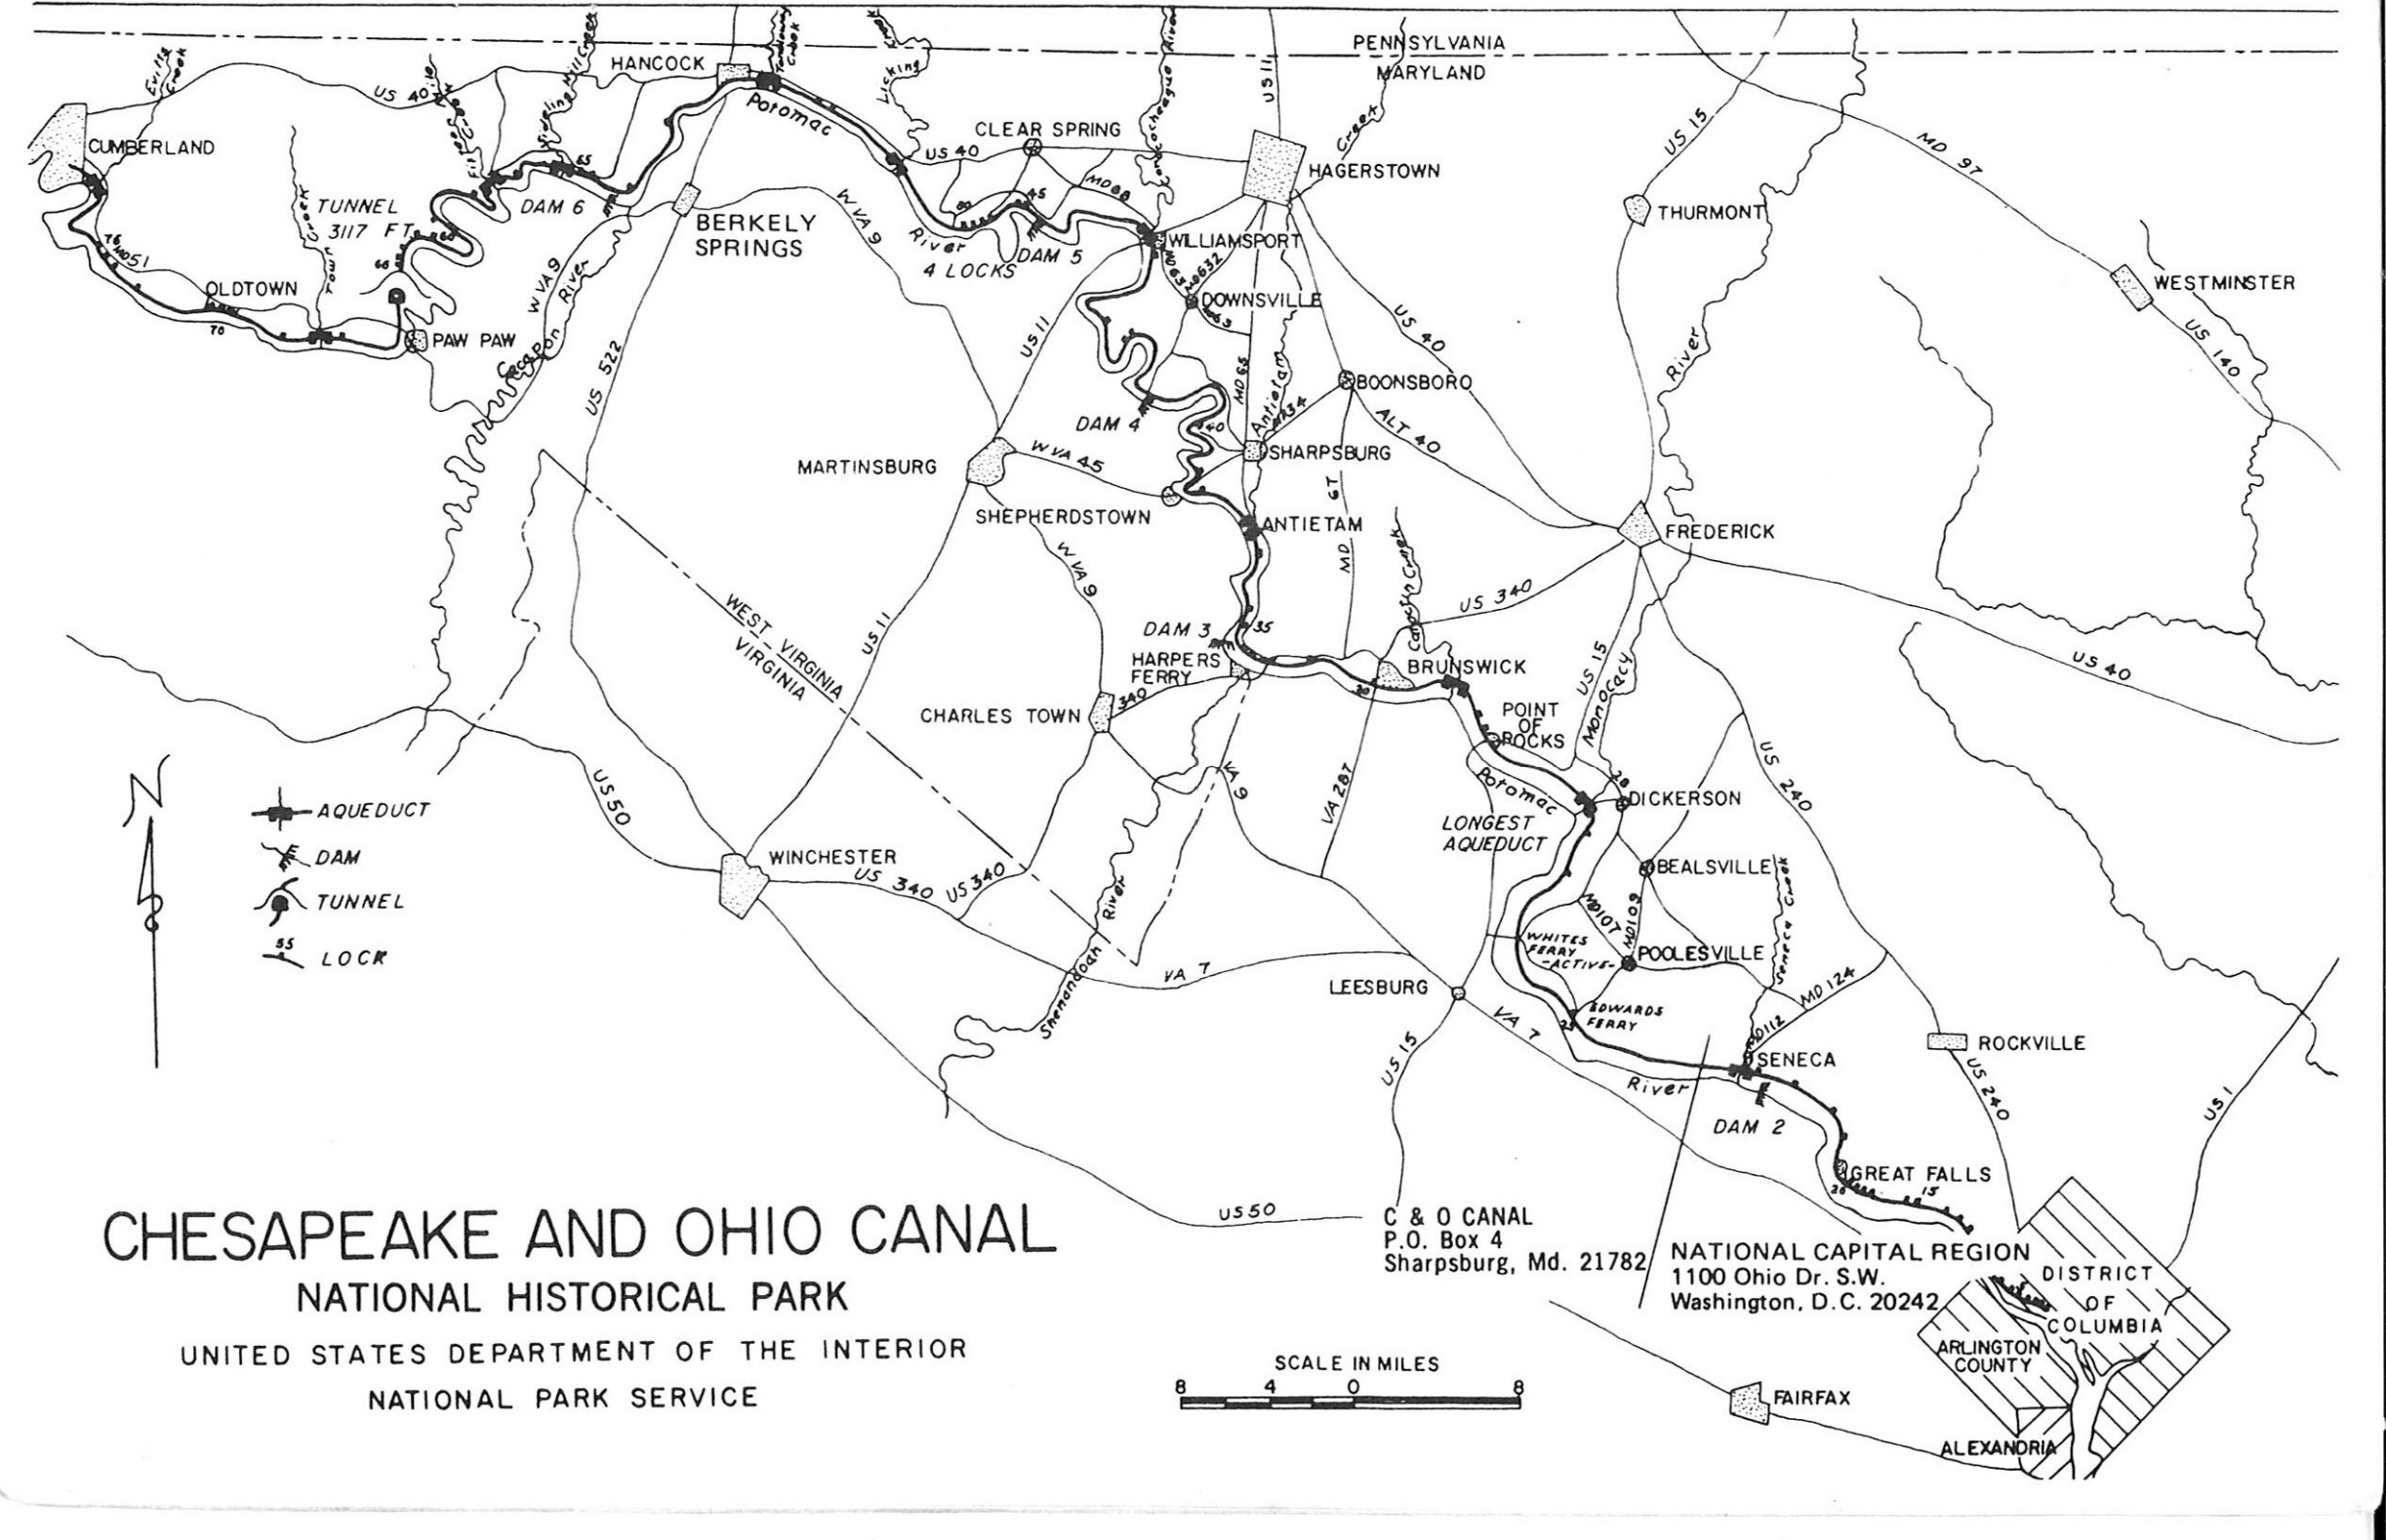
\includegraphics[height =7cm]{CroppedMapPic.png}
\end{center}


\end{block}
\begin{block}{}


\end{block}
\begin{block}{}
  
\end{block}
\end{column}
\separatorcolumn
\begin{column}{\colwidth}
\begin{block}{}


\end{block}
\begin{block}{Putting it All Together}

\end{block}
\end{column}
\separatorcolumn
\begin{column}{\colwidth}
\begin{block}{Putting it All Together (cotd.)}
\end{block}
\begin{block}{Conclusion}

\end{block}
\begin{block}{Acknowledgements}

\end{block}
\begin{block}{References}
bikecando.com\\
184 Miles of Adventure (book) 
\end{block}
\end{column}
\separatorcolumn
\end{columns}
\end{frame}
\end{document}
